\documentclass{../../Latex_Template/Homework/homework}
\usepackage[utf8]{inputenc}
\usepackage{float}

% Graphics Path
\graphicspath{ {images/} }

% CHANGE THE FOLLOW THREE LINES!
\newcommand{\hwname}{Wu, Bo-Run}
\newcommand{\hwstudentid}{r08942073}
\newcommand{\hwnum}{1}
\newcommand{\hwtype}{Homework}
\newcommand{\hwsection}{}
\newcommand{\hwlecture}{}
\newcommand{\hwclass}{FinTech}
\newcommand{\hwdate}{2020-11-16}

\begin{document}

\maketitle

\question*{Classification}
  \begin{alphaparts}
    \questionpart
    The model structure of DNN consists of three layers of Neural Network with
    28, 8 and 2 nodes respectively. During the grid search, I found that deeper
    network gets better results. But to avoid overfitting, I decided to pick 3
    layers to be the basic model structure of the DNN. Furthermore, the
    minibatch used for training is 512. The training accuracy and loss are shown
    below. 
    \begin{figure}[h]
      \centering
      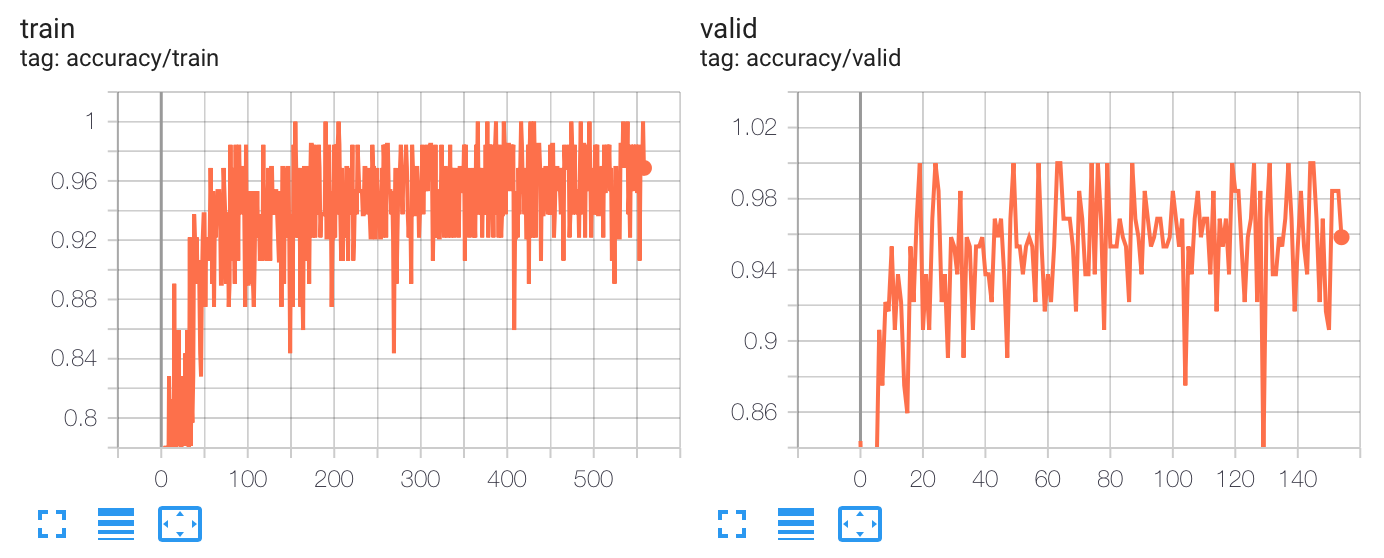
\includegraphics[width=0.5\linewidth]{Accuracy.png}
      \caption{Accuracy}
      \label{fig:accuracy}
    \end{figure}
        
    \begin{figure}[h]
      \centering
      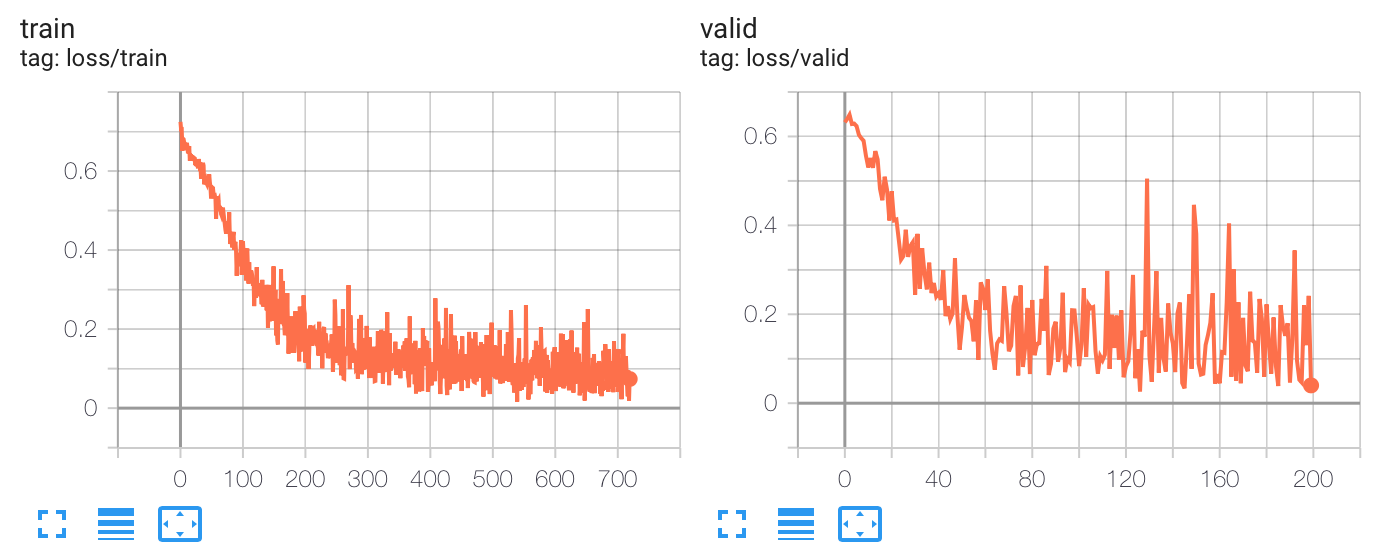
\includegraphics[width=0.5\linewidth]{Loss.png}
      \caption{Loss}
      \label{fig:loss}
    \end{figure}
        
    \questionpart
    The confusion matrix is plotted by one minibatch.
    \begin{figure}[h]
      \centering
      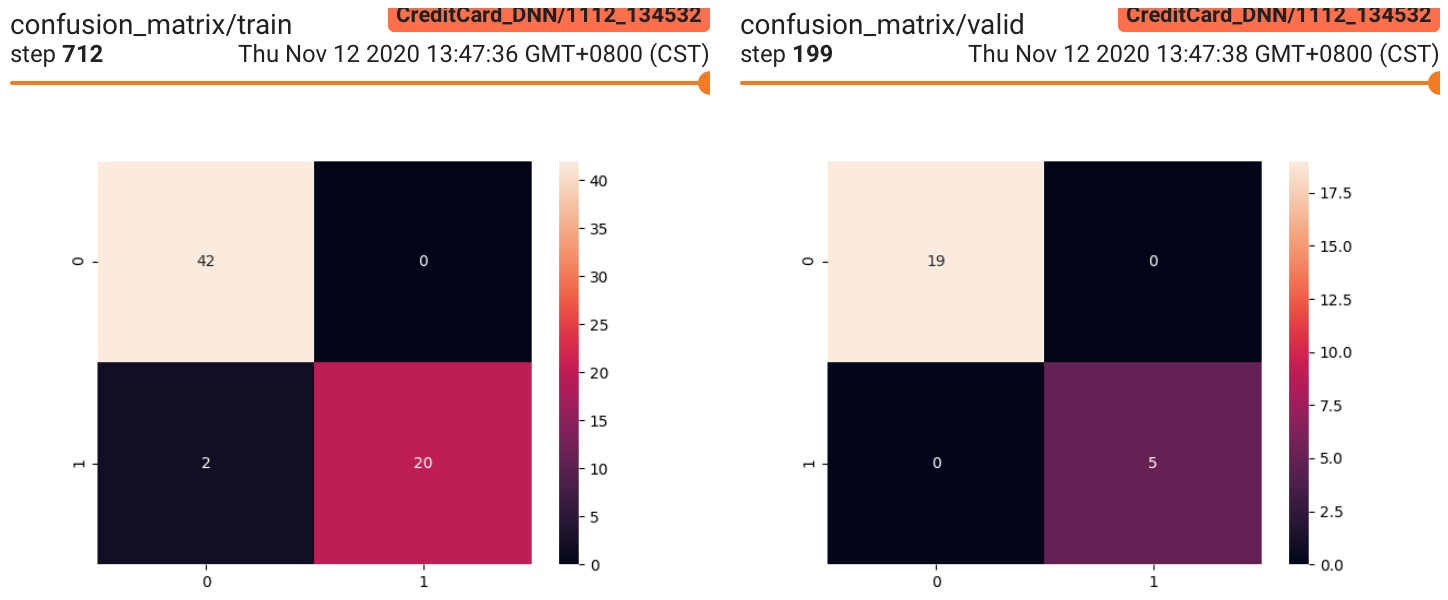
\includegraphics[width=0.5\linewidth]{Confusion_Matrix.png}
      \caption{Confusion Matrix}
      \label{fig:confusion_matrix}
    \end{figure}
        
    \questionpart
    Precision: 0.95, Recall: 0.87, F1 Score: 0.9
        
    \questionpart
    Decision tree uses a tree to classify the training data into different
    leaves according to the condition. Random forests are an ensemble learning
    method that operates by constructing a multitude of decision trees.
        
    \questionpart
    Decision tree: accuracy: 0.91, precision: 0.86, recall: 0.89, f1-score: 0.88
    Random forest: accuracy: 0.95, precision: 0.99, recall: 0.86, f1-score: 0.92
         
    \questionpart
    The figure of ROC Curve, Precision-Recall Curve and Lift Curve are shown
    below
    \begin{figure}[h]
      \centering
      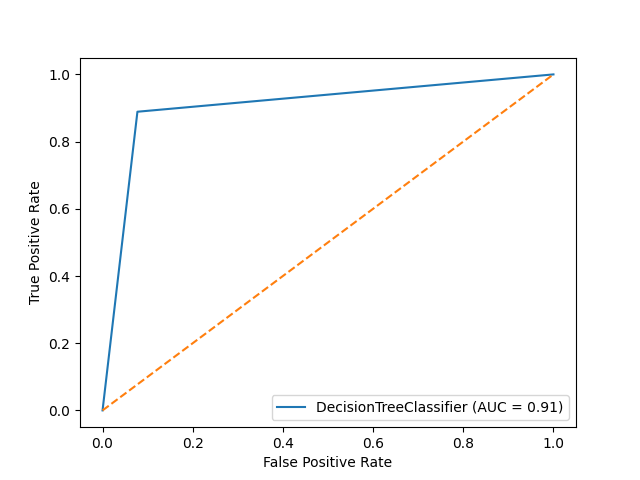
\includegraphics[width=0.5\linewidth]{DST_ROC.png}
      \caption{Decision Tree ROC Curve}
      \label{fig:DST_ROC.png}
    \end{figure}
          
    \begin{figure}[h]
      \centering
      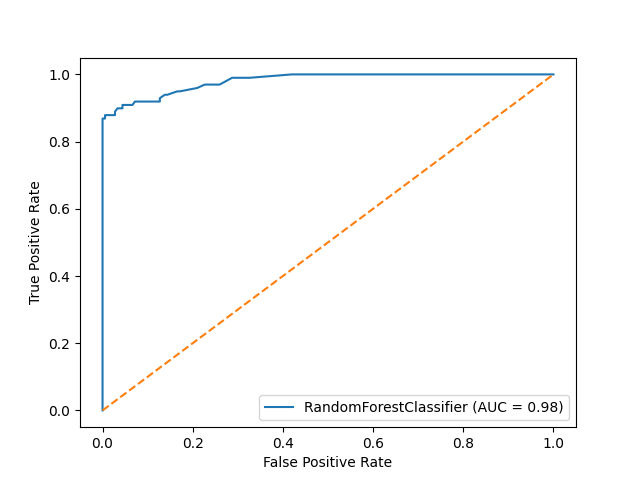
\includegraphics[width=0.5\linewidth]{RF_ROC.png}
      \caption{Random Forest ROC Curve}
      \label{fig:RF_ROC}
    \end{figure}
    
    \pagebreak
    
    \begin{figure}[h]
      \centering
      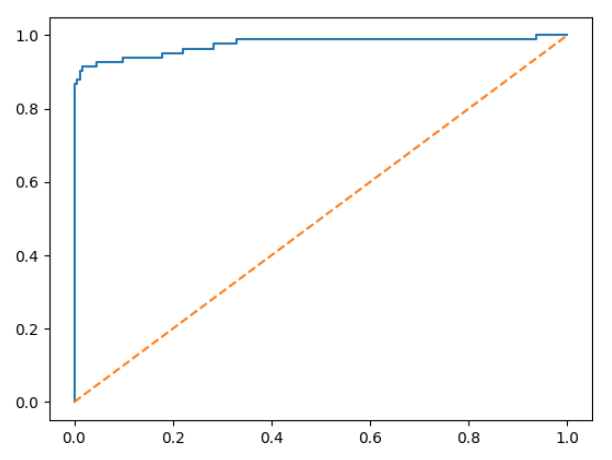
\includegraphics[width=0.5\linewidth]{DNN_ROC.png}
      \caption{DNN ROC Curve}
      \label{fig:DNN_ROC}
    \end{figure}

    \begin{figure}[h]
      \centering
      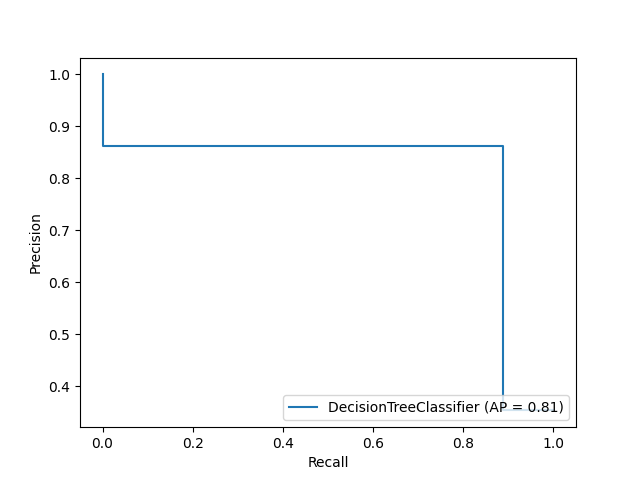
\includegraphics[width=0.5\linewidth]{DST_PRC.png}
      \caption{Decision Tree Precision Recall Curve}
      \label{fig:DST_PRC}
    \end{figure}
    
    \begin{figure}[h]
      \centering
      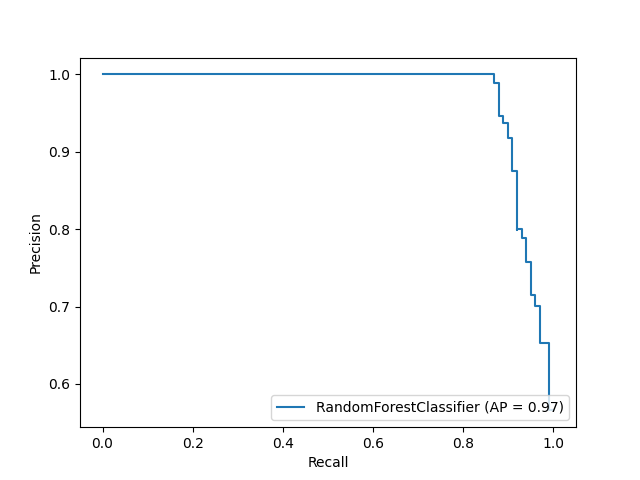
\includegraphics[width=0.5\linewidth]{RF_PRC.png}
      \caption{Random Forest Precision Recall Curve}
      \label{fig:RF_PRC}
    \end{figure}

    \begin{figure}[h]
      \centering
      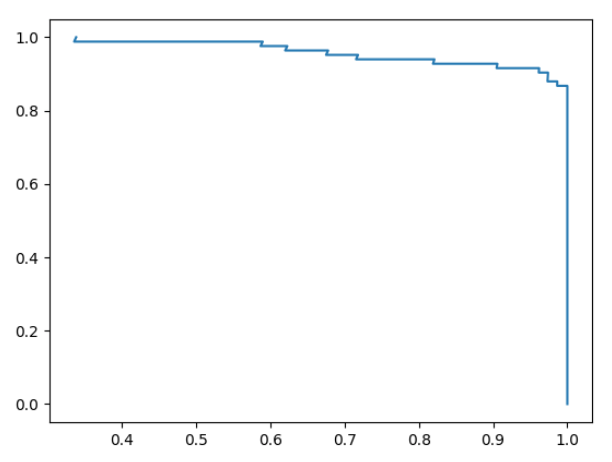
\includegraphics[width=0.5\linewidth]{DNN_PRC.png}
      \caption{DNN Precision Recall Curve}
      \label{fig:DNN_PRC}
    \end{figure}
    
    \pagebreak
  \end{alphaparts}
    

\question*{Lift Curve}
  \begin{figure}[h]
    \centering
    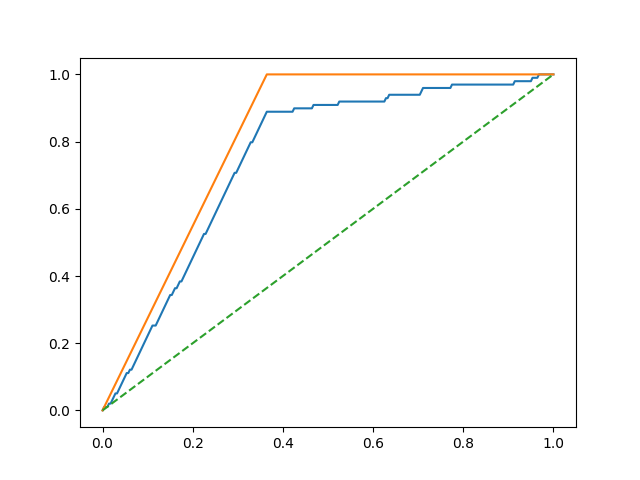
\includegraphics[width=0.5\linewidth]{DST_LIFT.png}
    \caption{Decision Tree Lift Curve}
    \label{fig:DNN_PRC}
  \end{figure}
  
  \begin{figure}[h]
    \centering
    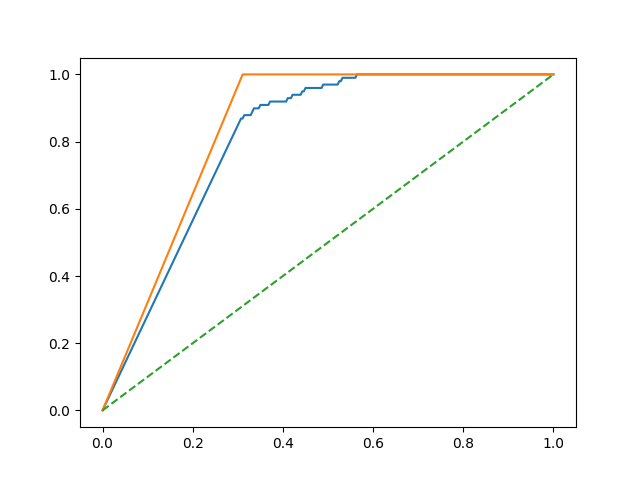
\includegraphics[width=0.5\linewidth]{RF_LIFT.png}
    \caption{Random Forest Lift Curve}
    \label{fig:RF_LIFT}
  \end{figure}
  
  \begin{figure}[h]
    \centering
    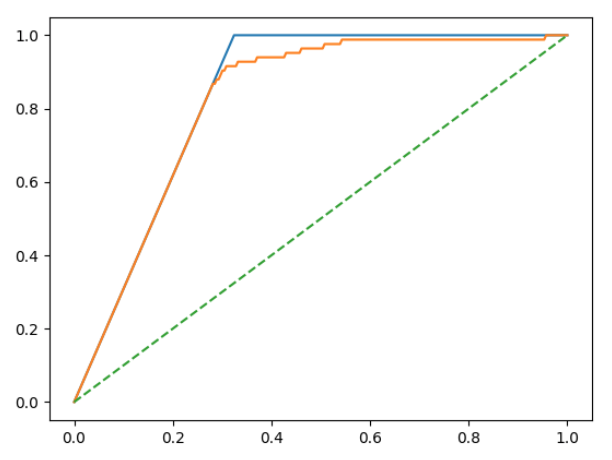
\includegraphics[width=0.5\linewidth]{DNN_LIFT.png}
    \caption{DNN LIFT Curve}
    \label{fig:DNN_LIFT}
  \end{figure}

\end{document}
